\section{Extracting recursive calls to statements}

This pass extracts recursive calls in the method body to separate statements
(\textit{LocalVariableDeclarationStatement}s\footnote{\url{https://docs.oracle.com/javase/specs/jls/se8/html/jls-14.html#jls-LocalVariableDeclarationStatement}}
with the method call as the
\textit{VariableInitializer}\footnote{\url{https://docs.oracle.com/javase/specs/jls/se8/html/jls-8.html#jls-VariableInitializer}}),
if the call is not already the \textit{VariableInitializer} of a \textit{LocalVariableDeclarationStatement} or the
right-hand side of an \textit{Assignment}\footnote{\url{https://docs.oracle.com/javase/specs/jls/se8/html/jls-15.html#jls-Assignment}}
having an \textit{ExpressionStatement}\footnote{\url{https://docs.oracle.com/javase/specs/jls/se8/html/jls-14.html#jls-ExpressionStatement}}
as parent. The pass does not affect recursive methods with \code{void} return type, because recursive calls to these
methods are already part of a separate \textit{ExpressionStatement}.

This code modification is necessary because the expression in which a recursive call may be embedded gets evaluated
only after returning from the recursive call. By separating the point of return from recursion from the following
computations, it becomes possible to jump in the method body to the statements after the call. An example is provided
in \labelindexref{Figure}{img:extract}.

\begin{figure}[htb]
    \makebox[\linewidth][c]{%
    \begin{subfigure}[b]{.5\textwidth}
        \centering
        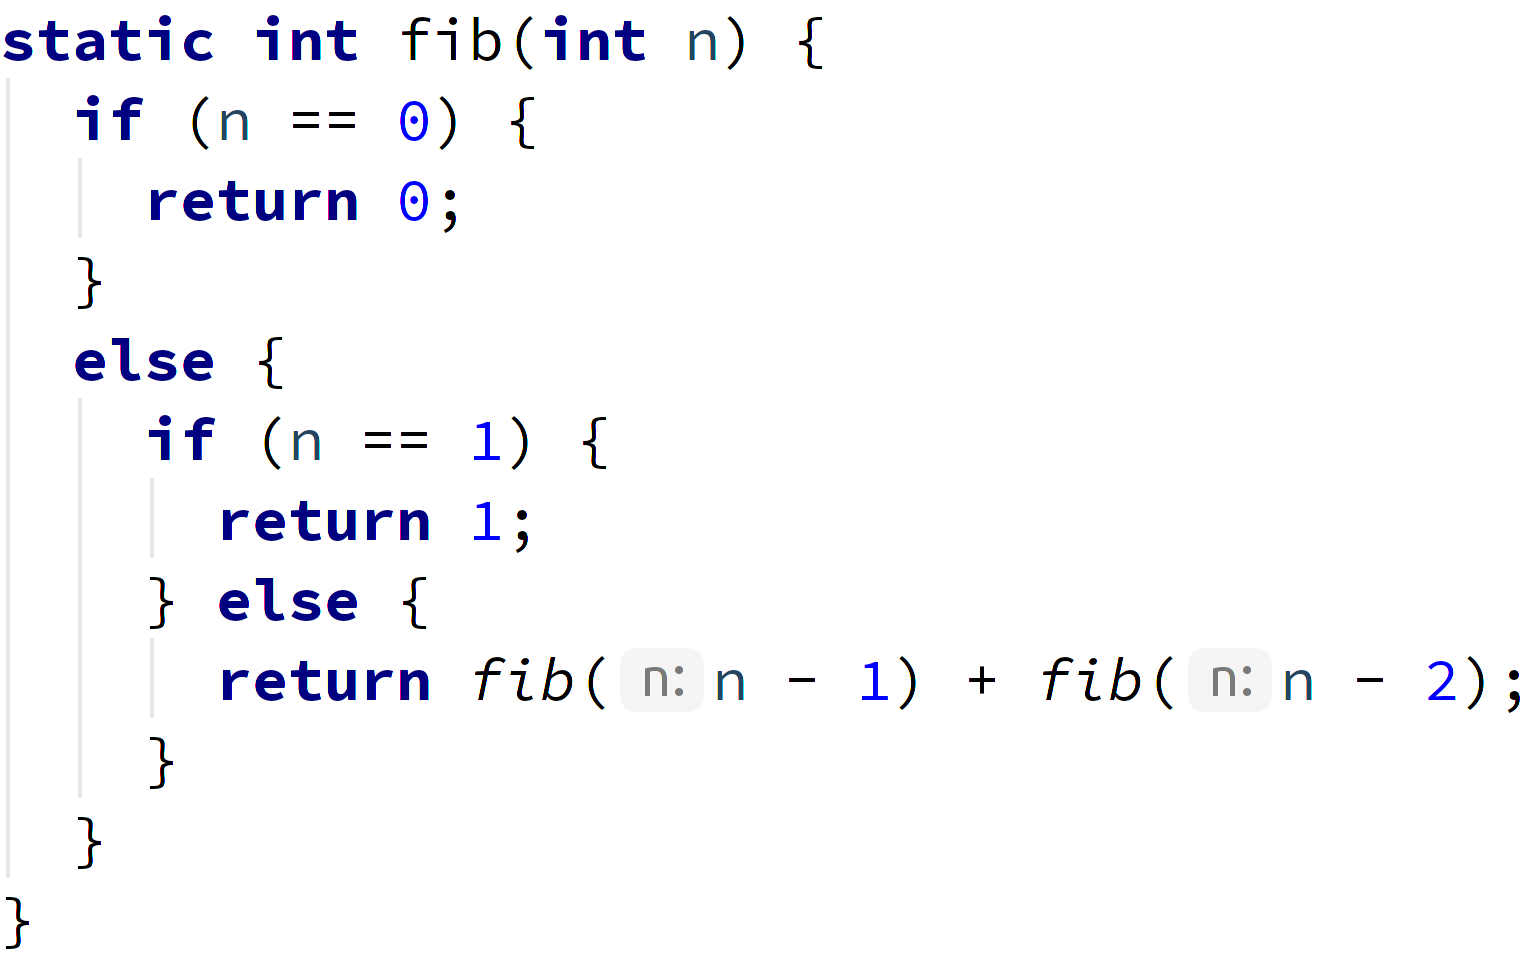
\includegraphics[height=1.44in]{src/img/replace-single-statements-with-block-statements-after-white.png}
        \caption{Before}
    \end{subfigure}%
    \begin{subfigure}[b]{.5\textwidth}
        \centering
        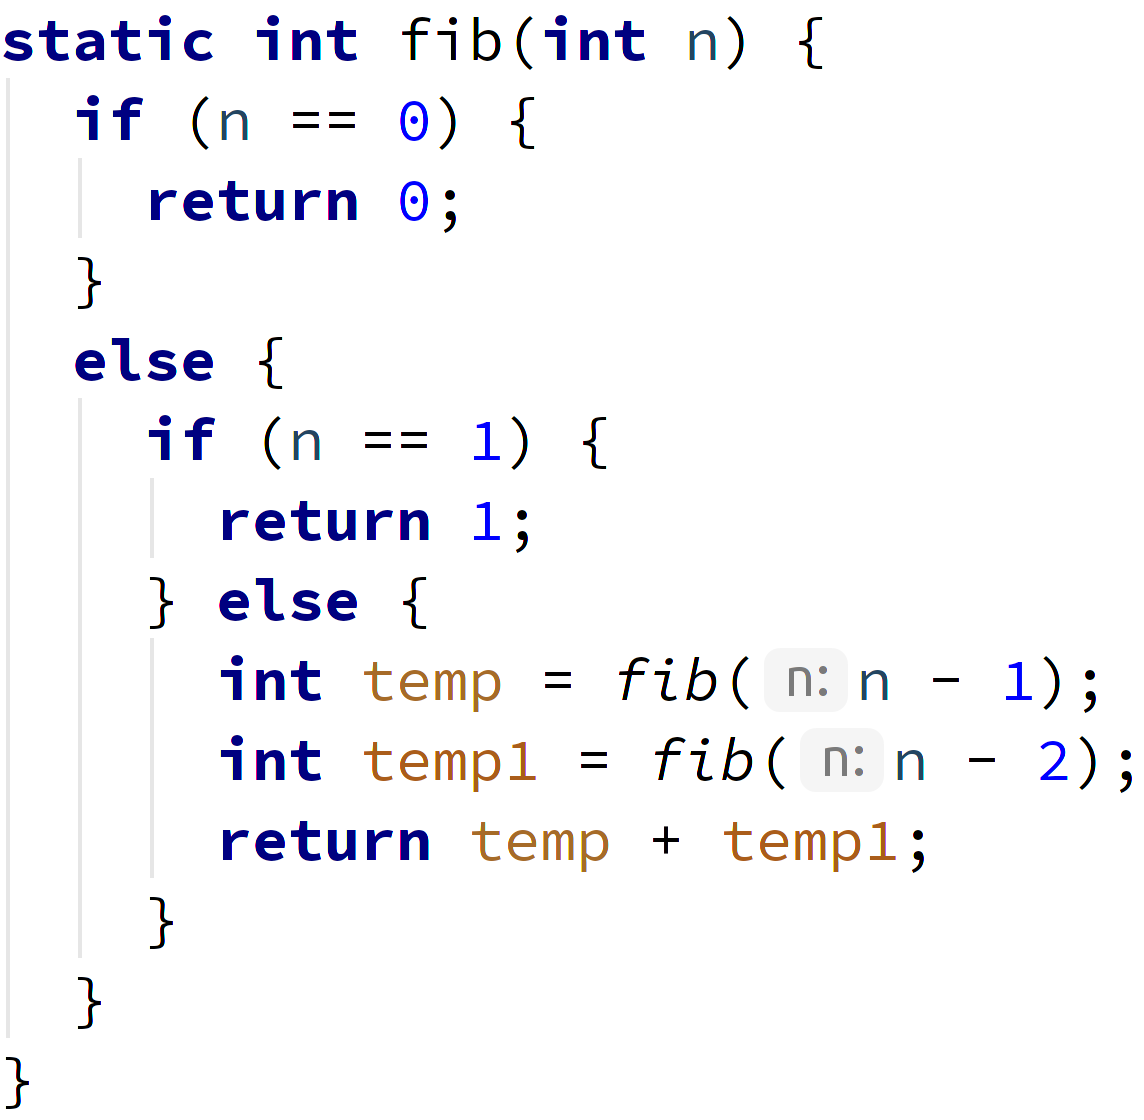
\includegraphics[height=1.68in]{src/img/extract-after-white.png}
        \caption{After}
    \end{subfigure}%
    }\\
    \caption{Extracting recursive calls to statements \label{img:extract}}
\end{figure}